\documentclass[12pt]{article}
\usepackage[a4paper, portrait, margin=2.5cm]{geometry}
\usepackage{tikz}  % For drawing diagrams
\usepackage{amsmath}  % For math symbols

\begin{document}

\begin{center}
    \Large \textbf{Perimeter Calculation Worksheet}
\end{center}

\vspace{10pt}
\noindent \textbf{Instructions:} \\
The diagram below shows a shape constructed by joining dots on a 1 cm grid. Calculate the perimeter of the shape by adding the lengths of all its sides. Assume each dot is spaced exactly 1 cm apart.

\vspace{10pt}

\begin{center}
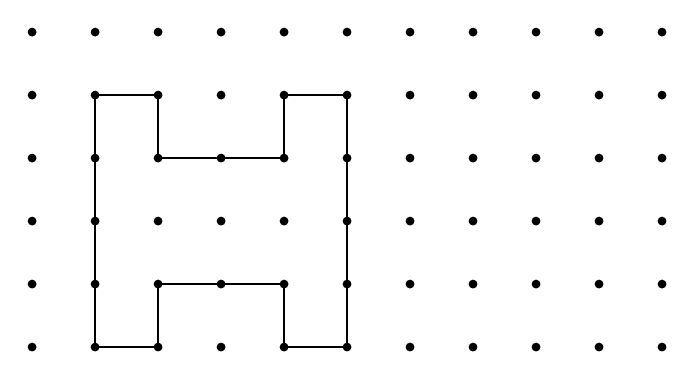
\begin{tikzpicture}[scale=0.8]

% Draw the 10x5 grid
\foreach \x in {0,1,...,10} {
    \foreach \y in {0,1,...,5} {
        \fill[black] (\x,\y) circle (2pt); % Fill each point with a black dot
    }
}

% Draw example shape (Modify this shape as needed)
\draw[thick] (1,0) -- (1,4)      % Left vertical line
              -- (2,4)            % Top right of the left rectangle
              -- (2,3)            % Move down to the crossbar
              -- (4,3)            % Move to the crossbar on the right
              -- (4,4)            % Move up to the top right corner
              -- (5,4)            % Move right to the top
              -- (5,0)            % Move down to the bottom right corner
              -- (4,0)            % Move left to the bottom of the right rectangle
              -- (4,1)            % Move up to the crossbar
              -- (2,1)            % Move left to the crossbar on the left
              -- (2,0)            % Move down to the bottom left corner
              -- (1,0)            % Close the shape at the bottom left corner
              -- cycle;

\end{tikzpicture}
\end{center}

\vspace{10pt}

\noindent \textbf{Question:}
\begin{enumerate}
    \item Calculate the perimeter of the shape in the diagram above. Write your working below:
    \vspace{6cm}  % Space for students to show their working
\end{enumerate}

\vfill

\end{document}
